%% This file was auto-generated by IPython.
%% Conversion from the original notebook file:
%% Exercise 6.ipynb
%%
\documentclass[a4paper, 12pt]{article}

%% This is the automatic preamble used by IPython.  Note that it does *not*
%% include a documentclass declaration. The documentclass is added at runtime
%% to the overall document.
\usepackage{fancyhdr}
\usepackage{amsmath}
\usepackage{amssymb}
\usepackage{graphicx}
\usepackage{ucs}
\usepackage[utf8x]{inputenc}

% needed for markdown enumerations to work
\usepackage{enumerate}

% Slightly bigger margins than the latex defaults
\usepackage{geometry}
\geometry{verbose,tmargin=3cm,bmargin=3cm,lmargin=2.5cm,rmargin=2.5cm}

% Define a few colors for use in code, links and cell shading
\usepackage{color}
\definecolor{orange}{cmyk}{0,0.4,0.8,0.2}
\definecolor{darkorange}{rgb}{.71,0.21,0.01}
\definecolor{darkgreen}{rgb}{.12,.54,.11}
\definecolor{myteal}{rgb}{.26, .44, .56}
\definecolor{gray}{gray}{0.45}
\definecolor{lightgray}{gray}{.95}
\definecolor{mediumgray}{gray}{.8}
\definecolor{inputbackground}{rgb}{.95, .95, .85}
\definecolor{outputbackground}{rgb}{.95, .95, .95}
\definecolor{traceback}{rgb}{1, .95, .95}

% Framed environments for code cells (inputs, outputs, errors, ...).  The
% various uses of \unskip (or not) at the end were fine-tuned by hand, so don't
% randomly change them unless you're sure of the effect it will have.
\usepackage{framed}

% remove extraneous vertical space in boxes
\setlength\fboxsep{0pt}

% codecell is the whole input+output set of blocks that a Code cell can
% generate.

% TODO: unfortunately, it seems that using a framed codecell environment breaks
% the ability of the frames inside of it to be broken across pages.  This
% causes at least the problem of having lots of empty space at the bottom of
% pages as new frames are moved to the next page, and if a single frame is too
% long to fit on a page, it will completely stop latex from compiling the
% document.  So unless we figure out a solution to this, we'll have to instead
% leave the codecell env. as empty.  I'm keeping the original codecell
% definition here (a thin vertical bar) for reference, in case we find a
% solution to the page break issue.

%% \newenvironment{codecell}{%
%%     \def\FrameCommand{\color{mediumgray} \vrule width 1pt \hspace{5pt}}%
%%    \MakeFramed{\vspace{-0.5em}}}
%%  {\unskip\endMakeFramed}

% For now, make this a no-op...
\newenvironment{codecell}{}

 \newenvironment{codeinput}{%
   \def\FrameCommand{\colorbox{inputbackground}}%
   \MakeFramed{\advance\hsize-\width \FrameRestore}}
 {\unskip\endMakeFramed}

\newenvironment{codeoutput}{%
   \def\FrameCommand{\colorbox{outputbackground}}%
   \vspace{-1.4em}
   \MakeFramed{\advance\hsize-\width \FrameRestore}}
 {\unskip\medskip\endMakeFramed}

\newenvironment{traceback}{%
   \def\FrameCommand{\colorbox{traceback}}%
   \MakeFramed{\advance\hsize-\width \FrameRestore}}
 {\endMakeFramed}

% Use and configure listings package for nicely formatted code
\usepackage{listingsutf8}
\lstset{
  language=python,
  inputencoding=utf8x,
  extendedchars=\true,
  aboveskip=\smallskipamount,
  belowskip=\smallskipamount,
  xleftmargin=2mm,
  breaklines=true,
  basicstyle=\small \ttfamily,
  showstringspaces=false,
  keywordstyle=\color{blue}\bfseries,
  commentstyle=\color{myteal},
  stringstyle=\color{darkgreen},
  identifierstyle=\color{darkorange},
  columns=fullflexible,  % tighter character kerning, like verb
}

% The hyperref package gives us a pdf with properly built
% internal navigation ('pdf bookmarks' for the table of contents,
% internal cross-reference links, web links for URLs, etc.)
\usepackage{hyperref}
\hypersetup{
  breaklinks=true,  % so long urls are correctly broken across lines
  colorlinks=true,
  urlcolor=blue,
  linkcolor=darkorange,
  citecolor=darkgreen,
  }

% hardcode size of all verbatim environments to be a bit smaller
\makeatletter
\g@addto@macro\@verbatim\small\topsep=0.5em\partopsep=0pt
\makeatother

% Prevent overflowing lines due to urls and other hard-to-break entities.
\sloppy

\newcommand{\HRule}{\rule{\linewidth}{0.5mm}}
\title{\bf Density Transformations \& ICA}
\author{Xugang Zhou \\ Fangzhou Yang}
\pagestyle{fancy}
\lhead{{\bf Machine Intelligence 2 SS2013}}
\rhead{Exercise 06}
\renewcommand{\headrulewidth}{0.4pt}

\begin{document}
\begin{titlepage}
\begin{center}
\vfill
\textsc{\LARGE Machine Intelligence 2}\\[1.5cm]
\textsc{\Large Exercise 06}\\[0.5cm]

\HRule \\[0.4cm]
{\huge \bfseries Density Transformations \& ICA}\\[0.4cm]
\HRule \\[1.5cm]
\begin{minipage}{0.4\textwidth}
\begin{flushleft} \large
\emph{Group Members:}\\
Xugang \textsc{Zhou}\\
Fangzhou \textsc{Yang}
\end{flushleft}
\end{minipage}
\begin{minipage}{0.4\textwidth}
\begin{flushright} \large
\emph{Tutor:} \\
Timm \textsc{Lochmann} \\
\end{flushright}
\end{minipage}
\vfill
{\large \today}\\
\end{center}
\end{titlepage}
\thispagestyle{fancy}


\section{6.1 Density Transformations}

Since
\[ f(x)dx = f(x(u)) \mid det \frac {\partial x(u)}{\partial u}\mid du \]
\[u = u(x) = e ^{-x} \] \[P_x(x) = f(x) = e^{-x}\]
\[P_u(u) = f(x(u))\mid det \frac {\partial x(u)}{\partial u}\mid\]

Thereforce \[ x = -\ln{u} \]
\[P_u(u) = x  * \mid -\frac{1}{x} \mid = 1 \]

\section{6.2 Random Number Generation}

Since
\[F(x)=\int_{-\infty}^x p(x) dx = \int_{-infty}^x \frac{1}{2b}e^{-\frac{|x-u|}{b}}dx \]
We get \[
z=F(x)=
\begin{cases} 1/2e^{-\frac{u-x}{b}} & x \le u \\\\ 
1-\frac{1}{2}e^{-\frac{x-u}{b}} & x > u
\end{cases}
\] Thereforce \[ x = F^{-1}(z) = 
\begin{cases} u+b\ln (2z) & 0 \le z \le \frac{1}{2} \\\\
u-b\ln (2-2z) & \frac{1}{2} < z \le 1
\end{cases}
\]

the random variable $z=F(x)$ is uniformly distributed on the interval
{[}0,1{]}

\begin{codecell}
\begin{codeinput}
\begin{lstlisting}
import matplotlib.pyplot as plt
#data generation with the formula above
u = 1
b = 1
size = 500
vectorX = [0 for i in range(size)]
z = random.uniform(0,1,size)
for i in range(500):
    if(z[i] > 0.5):
        vectorX[i] = u - b*math.log(2-2*z[i])
    else:
        vectorX[i] = u + b*math.log(2*z[i])

plt.clf()
plt.hist(z, bins=50, color='blue')
plt.title('histogram of generated Variable Z')
plt.show()

plt.clf()
plt.hist(vectorX, bins=50, color='blue')
plt.title('histogram of generated Variable X')
plt.show()


vectorL = random.laplace(1,1,size)
plt.hist(vectorL, bins=50, color='blue')
plt.title('histogram of Laplace Variable L')
plt.show()
\end{lstlisting}
\end{codeinput}
\begin{codeoutput}
\begin{center}
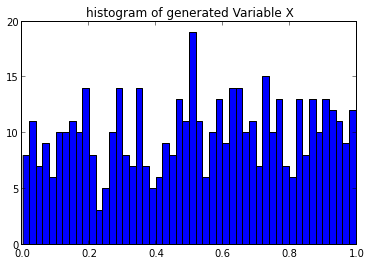
\includegraphics[width=0.7\textwidth]{Exercise_6_files/Exercise_6_fig_00.png}
\par
\end{center}
\begin{center}
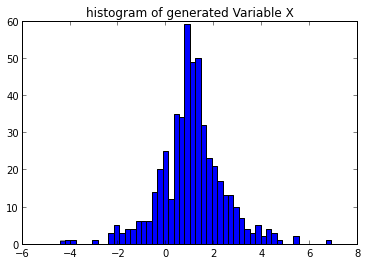
\includegraphics[width=0.7\textwidth]{Exercise_6_files/Exercise_6_fig_01.png}
\par
\end{center}
\begin{center}
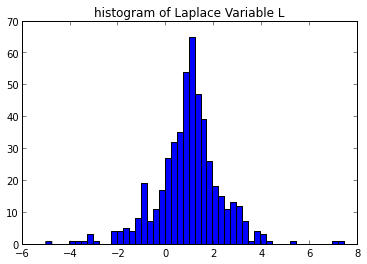
\includegraphics[width=0.7\textwidth]{Exercise_6_files/Exercise_6_fig_02.png}
\par
\end{center}
\end{codeoutput}
\end{codecell}
\section{6.3 ICA}

\subsection{Initialization}

\begin{codecell}
\begin{codeinput}
\begin{lstlisting}
from numpy import *
import random

#read data from pca2.csv
data01 = loadtxt('sounds/sound1.dat', unpack = True )
data02 = loadtxt('sounds/sound2.dat', unpack = True )
source = matrix([data01,data02])
length = source.shape[1]

#generate .wav files
import scipy.io.wavfile
def plotVoice(dataMatrix):
    length = dataMatrix.shape[1]
    fig1 = plt.figure(1)
    fig2 = plt.figure(2)
    ax1 = fig1.add_subplot(111)
    ax2 = fig2.add_subplot(111)
    ax1.plot(matrix.getA1(dataMatrix[0,:]))
    ax2.plot(matrix.getA1(dataMatrix[1,:]))
    plt.show()

def fileWriter(dataMatrix, file1, file2):
    normsig1 = asarray((2**16)*matrix.getA1(dataMatrix[0,:])/(max(matrix.getA1(dataMatrix[0,:]))-min(matrix.getA1(dataMatrix[0,:]))),int16) ## normalize before writing
    normsig2 = asarray((2**16)*matrix.getA1(dataMatrix[1,:])/(max(matrix.getA1(dataMatrix[1,:]))-min(matrix.getA1(dataMatrix[1,:]))),int16) ## normalize before writing
    scipy.io.wavfile.write(file1,8192,normsig1)
    scipy.io.wavfile.write(file2,8129,normsig2)
    
plotVoice(source)
fileWriter(source,'source1.wav','source2.wav')
    
\end{lstlisting}
\end{codeinput}
\begin{codeoutput}
\begin{center}
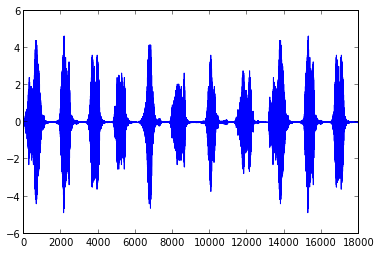
\includegraphics[width=0.7\textwidth]{Exercise_6_files/Exercise_6_fig_03.png}
\par
\end{center}
\begin{center}
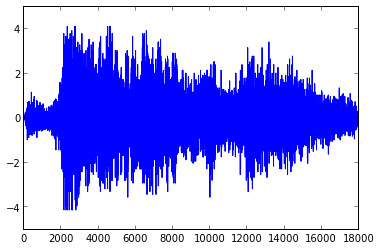
\includegraphics[width=0.7\textwidth]{Exercise_6_files/Exercise_6_fig_04.png}
\par
\end{center}
\end{codeoutput}
\end{codecell}
\begin{codecell}
\begin{codeinput}
\begin{lstlisting}
#create a random mixing matrix A and mix the sources: x = As
random.seed(100)
A = matrix([[random.random(),random.random()],[random.random(),random.random()]])
print "Matrix A is:"
print A
mix = A * source

plotVoice(mix)
fileWriter(mix,'mix1.wav','mix2.wav')


\end{lstlisting}
\end{codeinput}
\begin{codeoutput}
\begin{verbatim}
Matrix A is:
[[ 0.14566926  0.454927  ]
 [ 0.77078381  0.70551323]]
\end{verbatim}
\begin{center}
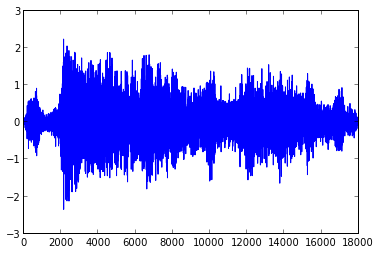
\includegraphics[width=0.7\textwidth]{Exercise_6_files/Exercise_6_fig_05.png}
\par
\end{center}
\begin{center}
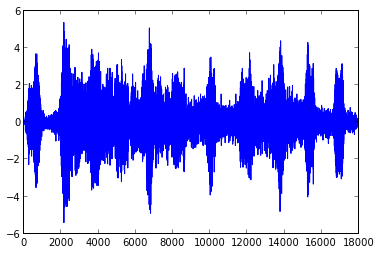
\includegraphics[width=0.7\textwidth]{Exercise_6_files/Exercise_6_fig_06.png}
\par
\end{center}
\end{codeoutput}
\end{codecell}
\begin{codecell}
\begin{codeinput}
\begin{lstlisting}
#permute the columns of N x p data matrix mix randomly
tmpCol = matrix([[0],[0]])
for i in range (length):
    colNo = random.randint(0, length-1)
    tmpCol = mix[:,colNo]
    mix[:,colNo] = mix[:,i]
    mix[:,i] = tmpCol
    
plotVoice(mix)
fileWriter(mix,'mix_per1.wav','mix_per2.wav')
\end{lstlisting}
\end{codeinput}
\begin{codeoutput}
\begin{center}
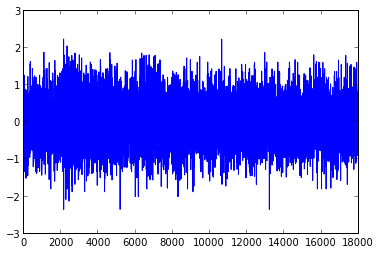
\includegraphics[width=0.7\textwidth]{Exercise_6_files/Exercise_6_fig_07.png}
\par
\end{center}
\begin{center}
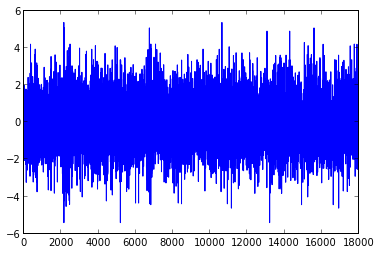
\includegraphics[width=0.7\textwidth]{Exercise_6_files/Exercise_6_fig_08.png}
\par
\end{center}
\end{codeoutput}
\end{codecell}
\begin{codecell}
\begin{codeinput}
\begin{lstlisting}
#Calculate the correlations between the sources and the mixtures
correlation = matrix([[0.],[0.]])
correlation[0,0] = corrcoef([source[0,i] for i in range (length)] , [mix[0,j] for j in range (length)])[0,1]
correlation[1,0] = corrcoef([source[1,i] for i in range (length)] , [mix[1,j] for j in range (length)])[0,1]    
print "Correlation between S and X:"
print correlation
\end{lstlisting}
\end{codeinput}
\begin{codeoutput}
\begin{verbatim}
Correlation between S and X:
[[ 0.11071182]
 [ 0.24131383]]
\end{verbatim}
\end{codeoutput}
\end{codecell}
\begin{codecell}
\begin{codeinput}
\begin{lstlisting}
#center the data to zero man
X = matrix([data01,data02])
for i in range (length):
    X[:,i] = mix[:,i] - mix.mean(1) 
    
#initialize the unmixing matrix W with random values
def init_W():
    random.seed(200)
    W = matrix([[random.random(), random.random()],[random.random(),random.random()]])
    return W
\end{lstlisting}
\end{codeinput}
\end{codecell}
\subsection{Optimization}

\[f(x) = \frac{1}{1+e ^{-x}} \]

\[f'(x) = f(x) * (1 - f(x)) \]

\[ f''(x) = f'(x) - 2f'(x)f(x) \]

\begin{codecell}
\begin{codeinput}
\begin{lstlisting}
#function f(x)
def f(x):
    return 1/(1+ math.exp(-x))

#function f''(x)/f'(x)
def fi(x):
    return 1 - 2*f(x)

#nomalization for matrix
def normalMatrix(m):
    for i in range(m.shape[0]):
        tmp = 0.
        for j in range(m.shape[1]):
            tmp += m[i,j] ** 2
        tmp = math.sqrt(tmp)
        for j in range(m.shape[1]):
            m[i,j] /= tmp
\end{lstlisting}
\end{codeinput}
\end{codecell}
\subsubsection{a.) Gradient Ascent}

\begin{codecell}
\begin{codeinput}
\begin{lstlisting}
W = init_W()
print "Init-Matrix W: "
print W
iteration = length * 1
rate_init =0.5

delta_W = matrix([[0.,0.],[0.,0.]])
plot_DW = []
for t in range(1 , iteration):
    alpha = t % length
    rate = rate_init / t  
    for i in range(2):
        sum_WikXk = 0.
        for k in range(2):
            sum_WikXk += W[i,k] * X[k,alpha]
        for j in range(2):
            inverse = W.getI()
            delta_W[i,j] = rate * ( inverse[j,i] + fi(sum_WikXk) * X[j,alpha] ) 
    W = W + delta_W 
    if(t % 1000 == 0):
        tmp = delta_W[0,0]**2 + delta_W[1,1]**2 + delta_W[0,1]**2 + delta_W[1,0]**2
        plot_DW.append(tmp)
    #print W
print "matrix W is:"
print W
print "after normalization:"
normalMatrix(W)
print W
\end{lstlisting}
\end{codeinput}
\begin{codeoutput}
\begin{verbatim}
Init-Matrix W: 
[[ 0.0456093   0.20344697]
 [ 0.70912398  0.1428485 ]]
matrix W is:
\end{verbatim}
\begin{verbatim}
[[-1.23568822  2.24189833]
 [ 2.88958884 -0.50818057]]
after normalization:
[[-0.48271158  0.87577939]
 [ 0.98488529 -0.17320788]]
\end{verbatim}
\end{codeoutput}
\end{codecell}
\begin{codecell}
\begin{codeinput}
\begin{lstlisting}
#recovery
ds = W * source

plotVoice(ds)
fileWriter(ds, 'recovery1.wav', 'recovery2.wav')
\end{lstlisting}
\end{codeinput}
\begin{codeoutput}
\begin{center}
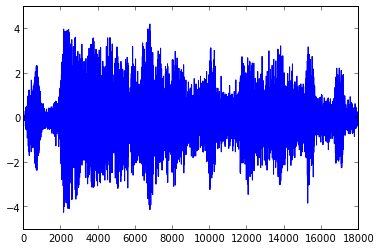
\includegraphics[width=0.7\textwidth]{Exercise_6_files/Exercise_6_fig_09.png}
\par
\end{center}
\begin{center}
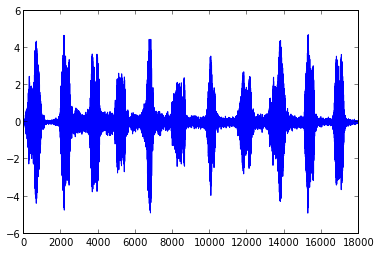
\includegraphics[width=0.7\textwidth]{Exercise_6_files/Exercise_6_fig_10.png}
\par
\end{center}
\end{codeoutput}
\end{codecell}
\begin{codecell}
\begin{codeinput}
\begin{lstlisting}
#Calculate the correlations between the true sources and the estimations
correlation = matrix([[0.],[0.]])
correlation[0,0] = corrcoef([source[0,i] for i in range (length)] , [ds[1,j] for j in range (length)])[0,1]
correlation[1,0] = corrcoef([source[1,i] for i in range (length)] , [ds[0,j] for j in range (length)])[0,1]    
print "Correlation between the true sources and the estimations:"
print correlation
\end{lstlisting}
\end{codeinput}
\begin{codeoutput}
\begin{verbatim}
Correlation between S and X:
[[ 0.98486963]
 [ 0.87570078]]
\end{verbatim}
\end{codeoutput}
\end{codecell}
\begin{codecell}
\begin{codeinput}
\begin{lstlisting}
#plot delta_W
fig = plt.figure()
ax = fig.add_subplot(111)
ax.set_xlabel('per 1000th update')
ax.plot([i+1 for i in range(len(plot_DW))],plot_DW)
plt.show()
\end{lstlisting}
\end{codeinput}
\begin{codeoutput}
\begin{center}
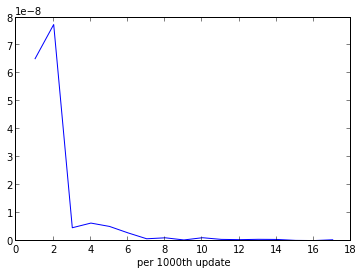
\includegraphics[width=0.7\textwidth]{Exercise_6_files/Exercise_6_fig_11.png}
\par
\end{center}
\end{codeoutput}
\end{codecell}
\begin{codecell}
\begin{codeinput}
\begin{lstlisting}
#Plot the density of the mixed, unmixed, and true signals.
ax=plt.subplot(321)
ax.hist(matrix.getA1(source[0,:]), bins=50, color='blue')
ax.set_title('histogram of 1st source')

ax=plt.subplot(322)
ax.hist(matrix.getA1(source[1,:]), bins=50, color='red')
ax.set_title('histogram of 2nd source')

ax=plt.subplot(323)
ax.hist(matrix.getA1(mix[0,:]), bins=50, color='blue')
ax.set_title('histogram of 1st mix')

ax=plt.subplot(324)
ax.hist(matrix.getA1(mix[1,:]), bins=50, color='red')
ax.set_title('histogram of 2st mix')

ax=plt.subplot(325)
ax.hist(matrix.getA1(ds[0,:]), bins=50, color='red')
ax.set_title('histogram of 1st ummix')

ax=plt.subplot(326)
ax.hist(matrix.getA1(ds[1,:]), bins=50, color='blue')
ax.set_title('histogram of 2nd unmix')

plt.show()
\end{lstlisting}
\end{codeinput}
\begin{codeoutput}
\begin{center}
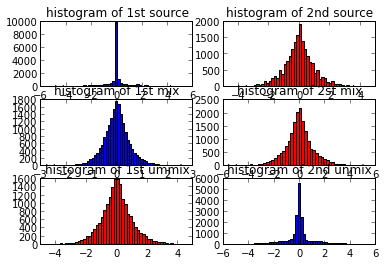
\includegraphics[width=0.7\textwidth]{Exercise_6_files/Exercise_6_fig_12.png}
\par
\end{center}
\end{codeoutput}
\end{codecell}
\subsubsection{b.) Natural Gradient}

\begin{codecell}
\begin{codeinput}
\begin{lstlisting}
W = init_W()
print "Init-Matrix W: "
print W
iteration = length * 1
rate_init =0.5

delta_W = matrix([[0.,0.],[0.,0.]])
plot_DW_natural = []
for t in range(1 , iteration):
    alpha = t % length
    rate = rate_init / t  
    for i in range(2):
        sum_WikXk = 0.
        for k in range(2):
            sum_WikXk += W[i,k] * X[k,alpha]
        for j in range(2):
            sum_Wlj = 0
            for l in range(2):
                if (l == i):
                    continue
                sum_WlkXk = 0
                for k in range (2):
                    sum_WlkXk += W[l,k] * X[k,alpha]
                sum_Wlj += sum_WlkXk
        delta_W[i,j] = rate * fi(sum_WikXk) * sum_Wlj
    W = W + delta_W 
    if(t % 1000 == 0):
        tmp = delta_W[0,0]**2 + delta_W[1,1]**2 + delta_W[0,1]**2 + delta_W[1,0]**2
        plot_DW_natural.append(tmp)
    #print W
print "matrix W is:"
print W
print "after normalization:"
normalMatrix(W)
print W
\end{lstlisting}
\end{codeinput}
\begin{codeoutput}
\begin{verbatim}
Init-Matrix W: 
[[ 0.0456093   0.20344697]
 [ 0.70912398  0.1428485 ]]
matrix W is:
\end{verbatim}
\begin{verbatim}
[[ 0.0456093   0.08026234]
 [ 0.70912398  0.02462701]]
after normalization:
[[ 0.4940561   0.86943003]
 [ 0.9993975   0.03470785]]
\end{verbatim}
\end{codeoutput}
\end{codecell}
\begin{codecell}
\begin{codeinput}
\begin{lstlisting}
#recovery
ds_natrual = W * source

plotVoice(ds_natrual)
fileWriter(ds_natrual, 'recovery_natual1.wav', 'recovery_natural2.wav')
\end{lstlisting}
\end{codeinput}
\begin{codeoutput}
\begin{center}
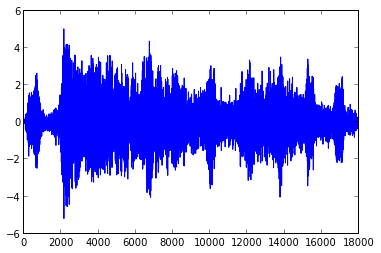
\includegraphics[width=0.7\textwidth]{Exercise_6_files/Exercise_6_fig_13.png}
\par
\end{center}
\begin{center}
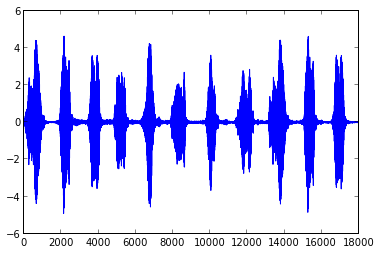
\includegraphics[width=0.7\textwidth]{Exercise_6_files/Exercise_6_fig_14.png}
\par
\end{center}
\end{codeoutput}
\end{codecell}
\begin{codecell}
\begin{codeinput}
\begin{lstlisting}
#Calculate the correlations between the true sources and the estimations
correlation_natural = matrix([[0.],[0.]])
correlation_natural[0,0] = corrcoef([source[0,i] for i in range (length)] , [ds_natrual[1,j] for j in range (length)])[0,1]
correlation_natural[1,0] = corrcoef([source[1,i] for i in range (length)] , [ds_natrual[0,j] for j in range (length)])[0,1]    
print "Correlation between the true sources and the estimations:"
print correlation_natural
\end{lstlisting}
\end{codeinput}
\begin{codeoutput}
\begin{verbatim}
Correlation between the true sources and the estimations:
[[ 0.99939718]
 [ 0.86964748]]
\end{verbatim}
\end{codeoutput}
\end{codecell}
\begin{codecell}
\begin{codeinput}
\begin{lstlisting}
#plot delta_W_natural
fig = plt.figure()
ax = fig.add_subplot(111)
ax.set_xlabel('natural gradient--per 1000th update')
ax.plot([i+1 for i in range(len(plot_DW_natural))],plot_DW_natural)
plt.show()
\end{lstlisting}
\end{codeinput}
\begin{codeoutput}
\begin{center}
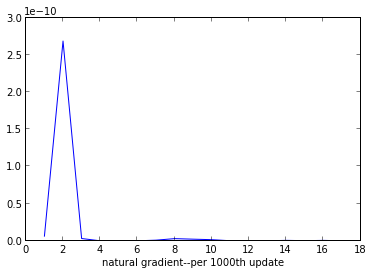
\includegraphics[width=0.7\textwidth]{Exercise_6_files/Exercise_6_fig_15.png}
\par
\end{center}
\end{codeoutput}
\end{codecell}
\begin{codecell}
\begin{codeinput}
\begin{lstlisting}
#Plot the density of the mixed, unmixed, and true signals.
ax=plt.subplot(321)
ax.hist(matrix.getA1(source[0,:]), bins=50, color='blue')
ax.set_title('histogram of 1st source')

ax=plt.subplot(322)
ax.hist(matrix.getA1(source[1,:]), bins=50, color='red')
ax.set_title('histogram of 2nd source')

ax=plt.subplot(323)
ax.hist(matrix.getA1(mix[0,:]), bins=50, color='blue')
ax.set_title('histogram of 1st mix')

ax=plt.subplot(324)
ax.hist(matrix.getA1(mix[1,:]), bins=50, color='red')
ax.set_title('histogram of 2st mix')

ax=plt.subplot(325)
ax.hist(matrix.getA1(ds_natrual[0,:]), bins=50, color='red')
ax.set_title('histogram of 1st ummix')

ax=plt.subplot(326)
ax.hist(matrix.getA1(ds_natrual[1,:]), bins=50, color='blue')
ax.set_title('histogram of 2nd unmix')

plt.show()
\end{lstlisting}
\end{codeinput}
\begin{codeoutput}
\begin{center}
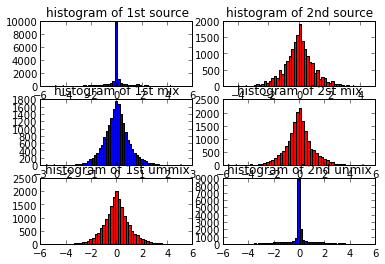
\includegraphics[width=0.7\textwidth]{Exercise_6_files/Exercise_6_fig_16.png}
\par
\end{center}
\end{codeoutput}
\end{codecell}
\subsubsection{Comparison of two learning methods}

\begin{codecell}
\begin{codeinput}
\begin{lstlisting}
ax=plt.subplot(211)
ax.set_title('regular gradient')
ax.plot([i+1 for i in range(len(plot_DW))],plot_DW)

ax=plt.subplot(212)
ax.set_title('natrual gradient')
ax.plot([i+1 for i in range(len(plot_DW_natural))],plot_DW_natural)
plt.show()
\end{lstlisting}
\end{codeinput}
\begin{codeoutput}
\begin{center}
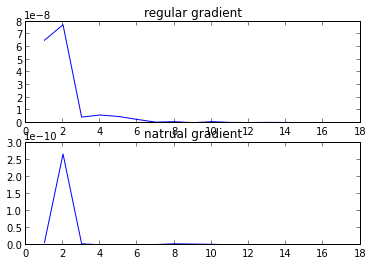
\includegraphics[width=0.7\textwidth]{Exercise_6_files/Exercise_6_fig_17.png}
\par
\end{center}
\end{codeoutput}
\end{codecell}
As we can see from the figure above, the natural gradient can get a
convergence point much faster.

\subsubsection{Comparison after whitening the Data}

\begin{codecell}
\begin{codeinput}
\begin{lstlisting}
#function to get the covariance matrix
def get_CoMatrix(data, dimension):
    C = [[0. for i in range(dimension)] for j in range(dimension)]
    p = data.shape[1]
    m = mix.mean(1)
    for i in range(dimension):
        for j in range(dimension):
            for a in range(p):
                C[i][j] += ( (data[i,a] - m[i,0]) * (data[j,a] - m[j,0]) )/p
    return C

#function to get eigenvalues and eigenvectors
def get_PC(data, dimension, nume):
    C = get_CoMatrix(data, dimension)   
    if nume == dimension:
        evals, evecs = np.linalg.eig(asmatrix(C))
    else:
        evals, evecs = sp.sparse.linalg.eigs(asmatrix(C), k = nume)
    return evals, evecs

evals, evecs = get_PC(X, 2, 2)
print evals
print evecs
E = matrix(evecs)
Dd = matrix(np.diag([ 1/math.sqrt(evals[i]) for i in range(2)]))
Z =(( X.T * E) * Dd).T
print 'after whitening:'
print Z
\end{lstlisting}
\end{codeinput}
\begin{codeoutput}
\begin{verbatim}
[ 0.05006899  1.35363586]
[[-0.92229698 -0.38648192]
 [ 0.38648192 -0.92229698]]
after whitening:
[[ 0.01834547  0.01844986  0.26840202 ..., -0.61824489  0.01844411
   0.01834547]
 [-0.00210848 -0.00199554  0.19219774 ...,  0.65723508  0.00203564
  -0.00210848]]
\end{verbatim}
\end{codeoutput}
\end{codecell}
a.do Regular gradient with whitened data

\begin{codecell}
\begin{codeinput}
\begin{lstlisting}
W = init_W()
print "Init-Matrix W: "
print W
iteration = length * 1
rate_init =0.5

delta_W = matrix([[0.,0.],[0.,0.]])
plot_DW = []
for t in range(1 , iteration):
    alpha = t % length
    rate = rate_init / t  
    for i in range(2):
        sum_WikXk = 0.
        for k in range(2):
            sum_WikXk += W[i,k] * Z[k,alpha]
        for j in range(2):
            inverse = W.getI()
            delta_W[i,j] = rate * ( inverse[j,i] + fi(sum_WikXk) * Z[j,alpha] ) 
    W = W + delta_W 
    if(t % 1000 == 0):
        tmp = delta_W[0,0]**2 + delta_W[1,1]**2 + delta_W[0,1]**2 + delta_W[1,0]**2
        plot_DW.append(tmp)
    #print W
print "matrix W is:"
print W
print "after normalization:"
normalMatrix(W)
print W
\end{lstlisting}
\end{codeinput}
\begin{codeoutput}
\begin{verbatim}
Init-Matrix W: 
[[ 0.0456093   0.20344697]
 [ 0.70912398  0.1428485 ]]
matrix W is:
\end{verbatim}
\begin{verbatim}
[[-0.16409082  2.23398162]
 [ 1.78681701  0.03664664]]
after normalization:
[[-0.07325483  0.99731326]
 [ 0.99978975  0.02050514]]
\end{verbatim}
\end{codeoutput}
\end{codecell}
b.do Natural gradient with whitened data

\begin{codecell}
\begin{codeinput}
\begin{lstlisting}
W = init_W()
print "Init-Matrix W: "
print W
iteration = length * 1
rate_init =0.5

delta_W = matrix([[0.,0.],[0.,0.]])
plot_DW_natural = []
for t in range(1 , iteration):
    alpha = t % length
    rate = rate_init / t  
    for i in range(2):
        sum_WikXk = 0.
        for k in range(2):
            sum_WikXk += W[i,k] * Z[k,alpha]
        for j in range(2):
            sum_Wlj = 0
            for l in range(2):
                if (l == i):
                    continue
                sum_WlkXk = 0
                for k in range (2):
                    sum_WlkXk += W[l,k] * Z[k,alpha]
                sum_Wlj += sum_WlkXk
        delta_W[i,j] = rate * fi(sum_WikXk) * sum_Wlj
    W = W + delta_W 
    if(t % 1000 == 0):
        tmp = delta_W[0,0]**2 + delta_W[1,1]**2 + delta_W[0,1]**2 + delta_W[1,0]**2
        plot_DW_natural.append(tmp)
    #print W
print "matrix W is:"
print W
print "after normalization:"
normalMatrix(W)
print W
\end{lstlisting}
\end{codeinput}
\begin{codeoutput}
\begin{verbatim}
Init-Matrix W: 
[[ 0.0456093   0.20344697]
 [ 0.70912398  0.1428485 ]]
matrix W is:
\end{verbatim}
\begin{verbatim}
[[ 0.0456093   0.08508957]
 [ 0.70912398  0.03919878]]
after normalization:
[[ 0.47242747  0.88136955]
 [ 0.99847568  0.05519349]]
\end{verbatim}
\end{codeoutput}
\end{codecell}
\begin{codecell}
\begin{codeinput}
\begin{lstlisting}
ax=plt.subplot(211)
ax.set_title('regular gradient')
ax.plot([i+1 for i in range(len(plot_DW))],plot_DW)

ax=plt.subplot(212)
ax.set_title('natrual gradient')
ax.plot([i+1 for i in range(len(plot_DW_natural))],plot_DW_natural)
plt.show()
\end{lstlisting}
\end{codeinput}
\begin{codeoutput}
\begin{center}
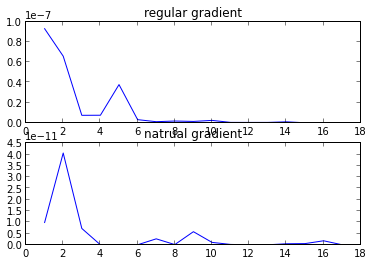
\includegraphics[width=0.7\textwidth]{Exercise_6_files/Exercise_6_fig_18.png}
\par
\end{center}
\end{codeoutput}
\end{codecell}
As we can see, after data whitening, the natural gradient takes much
longer time to get the convergence, while the convergence speed of
regular gradient stays the same.

\end{document}
